\documentclass[10pt]{article}
\usepackage{graphicx} % needed for including graphics e.g. EPS, PS
\usepackage{fancyhdr}
\usepackage[section]{placeins}
\usepackage{subfigure}
\topmargin -1.5cm        % read Lamport p.163
\oddsidemargin -0.37cm   % read Lamport p.163
\evensidemargin -0.25cm  % same as oddsidemargin but for left-hand pages
\textwidth 16.59cm \textheight 24.5cm
\pagestyle{fancy}       % Uncomment if don't want page numbers
\parskip 7.2pt           % sets spacing between paragraphs
%\renewcommand{\baselinestretch}{1.5} % Uncomment for 1.5 spacing between lines
\parindent 0pt       % sets leading space for paragraphs
\lhead{} \chead{\leftmark} \rhead{\thepage}
  \lfoot{}\cfoot{\thepage} \rfoot{}

\begin{document}
\title{Network Performance Analysis - Lab2}
\maketitle
\section*{Things to note}
We note that the average in the system which includes the packet
being served is given by

$$
\textrm{Average in the system}=\frac{\rho}{1-\rho}
$$

we also consider that the number being serviced in the system is
given by $\rho$ so the total in the queue is given by

\begin{eqnarray}
\overline{Q}&=&\frac{\rho}{1-\rho}-\rho\\
&=&\frac{\rho-(1-\rho)\rho}{1-\rho}\\
&=&\frac{\rho-\rho+\rho^2}{1-\rho}\\
&=&\frac{\rho^2}{1-\rho}
\end{eqnarray}
\section*{Question 1}
Simplex-link = Type of link in this case simplex which means in one direction.\\
\$node1 = the from node\\
\$node2 = the too node\\
8 kB = the bandwidth\\
0 ms = the time this takes to traverse the gap\\
Droptail = means that is the package is bigger than this then it
drops the rest of it.\\
\\
Following is a plot of the example of the queue running
\begin{figure}[h]
\centering
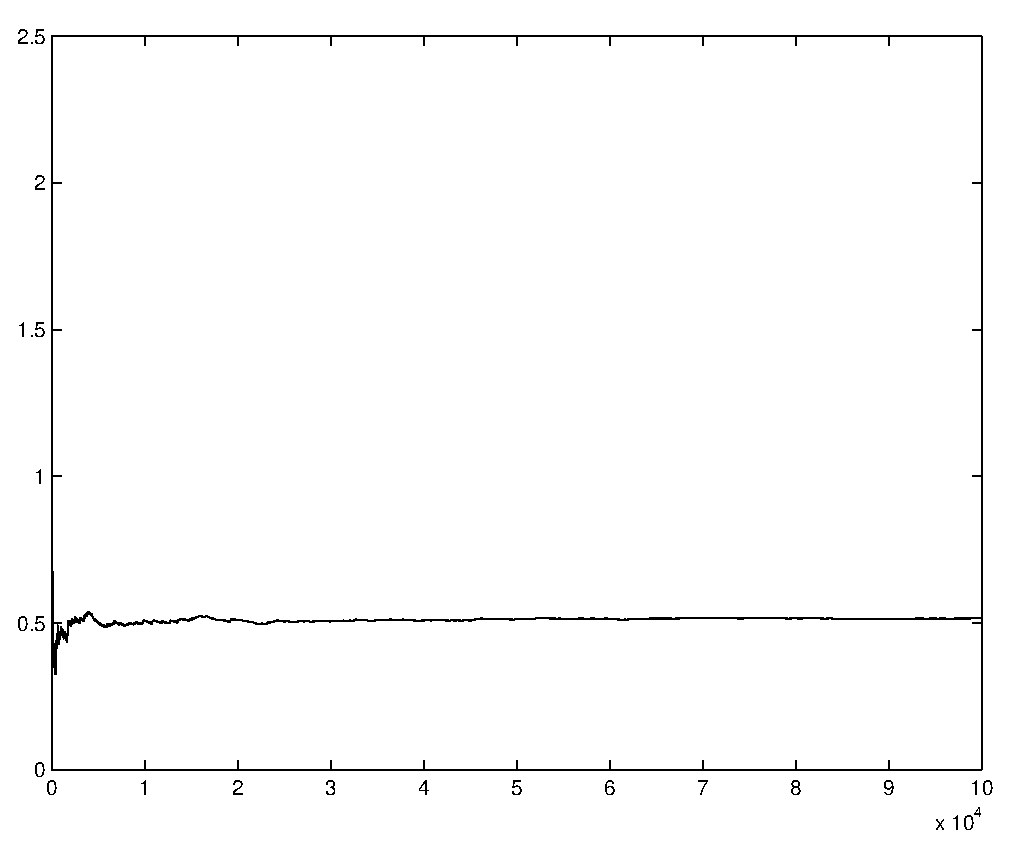
\includegraphics[height=6cm]{fig2.eps}
\caption{Figure of queue for question1}
\end{figure}

Running the queue for $\lambda=1$ and Packet length $\bar{X}=
\frac{1}{2}$ then theoretically

$$
\rho=\lambda\bar{X}=\frac{1}{2}
$$
$$
\left<k\right>_{p(k)}=\frac{\rho^2}{1-\rho}=\frac{(\frac{1}{2})^2}{1-\frac{1}{2}}=\frac{\frac{1}{4}}{\frac{1}{2}}=\frac{1}{2}
$$

The value in practice was also 0.5.


Running the queue for $\lambda=1.9$ and Packet length $\bar{X}=
\frac{1}{2}$ then theoretically

$$
\rho=\lambda\bar{X}=\frac{1.9}{2}=\frac{19}{20}
$$
$$
\left<k\right>_{p(k)}=\frac{\rho^2}{1-\rho}=\frac{(\frac{19}{20})^2}{1-\frac{19}{20}}=\frac{\frac{361}{400}}{\frac{1}{20}}=\frac{361}{20}=18.05
$$


The value in practice was 31 but theoretically it was 18.05.
\FloatBarrier
\section*{Question 2}
Coding question with a plot where the aim was for the student to
learn a little how the program works.

\section*{Question 3}
The architecture takes the following form
\begin{figure}[h]
\centering
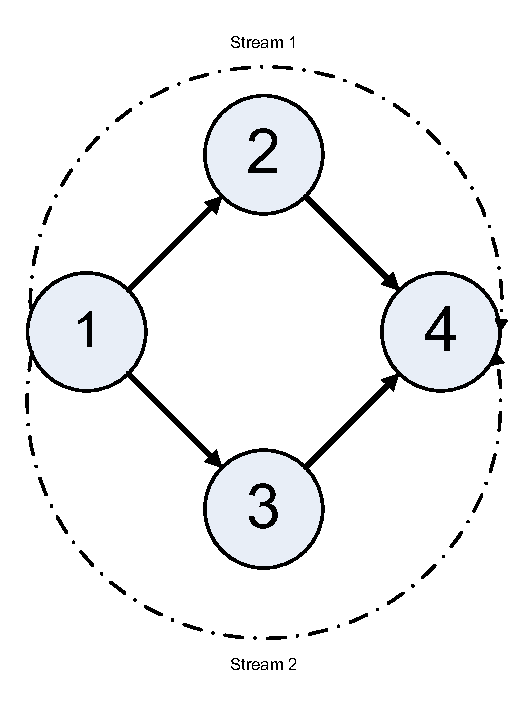
\includegraphics[height=6cm]{figQ3.eps}
\caption{Diagram of queue for question 3. Note the full lines are
the connections and the dotted line represent the streams.}
\end{figure}
\FloatBarrier
 We should note that for this architecture when
considering Kleinrock independence assumption we need to think in
terms of the streams. For this model we can see that we have two
streams of information, one stream goes from state 1 to state 2 to
state 4. The second stream moves from state 1 to state 3 to state
4. This has an effect when we consider the value of birthrate
$\lambda$ for each stream. Consider that
$$
\lambda=\lambda_1+\lambda_2
$$

and we know that both streams have equal birthrates, as such it is
easy to see that the birthrate value for one particular stream is
given by

$ \lambda_i=\frac{\lambda}{2}$.
\subsection*{Question 3 a}


For the base case $\lambda_i=1$, $\mu=2$ as effectively all the
links are equal then for each link

$$
\rho=\frac{\lambda}{\mu}=\frac{1}{2}=0.5
$$

so
$$
\overline{Q}_Q=\frac{\rho^2}{1-\rho}=\frac{0.5^2}{1-0.5}=0.5
$$

\subsection*{Question 3bi}
\begin{figure}[h]
\centering
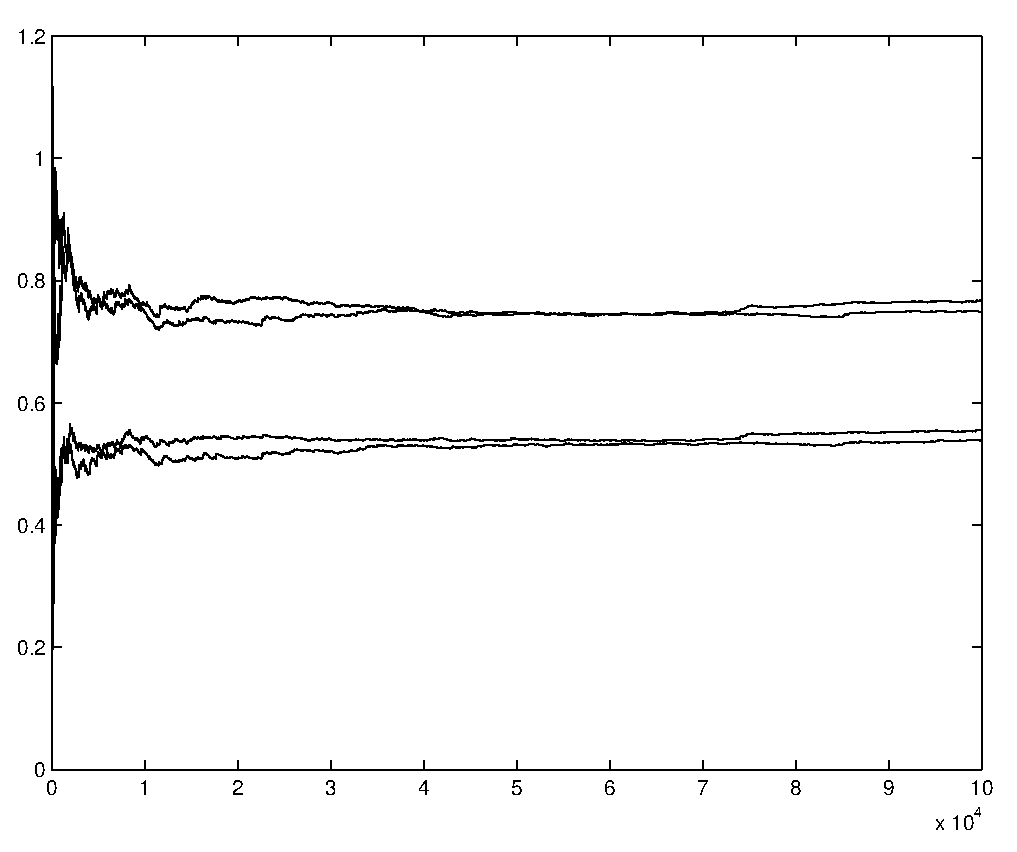
\includegraphics[height=6cm]{4bi.eps}
\caption{Figure of queue for question1}
\end{figure}
For the base case $\lambda_i=1$, $\mu=2$ as effectively all the
links are equal then for each link

$$
\rho=\frac{\lambda}{\mu}=\frac{1}{2}=0.5
$$

so
$$
\overline{Q}_Q=\frac{\rho^2}{1-\rho}=\frac{0.5^2}{1-0.5}=0.5
$$


\FloatBarrier

What we actually get for each queue is

$ q_1=0.4838 $ \\ $ q_2=0.5235 $ \\ $ q_3=0.7769 $ \\ $ q_4=0.8811
$

Here the analytical calculations are quite close to the values
obtained in practice.

\subsection{Question 3bii}
\begin{figure}[h]
\centering
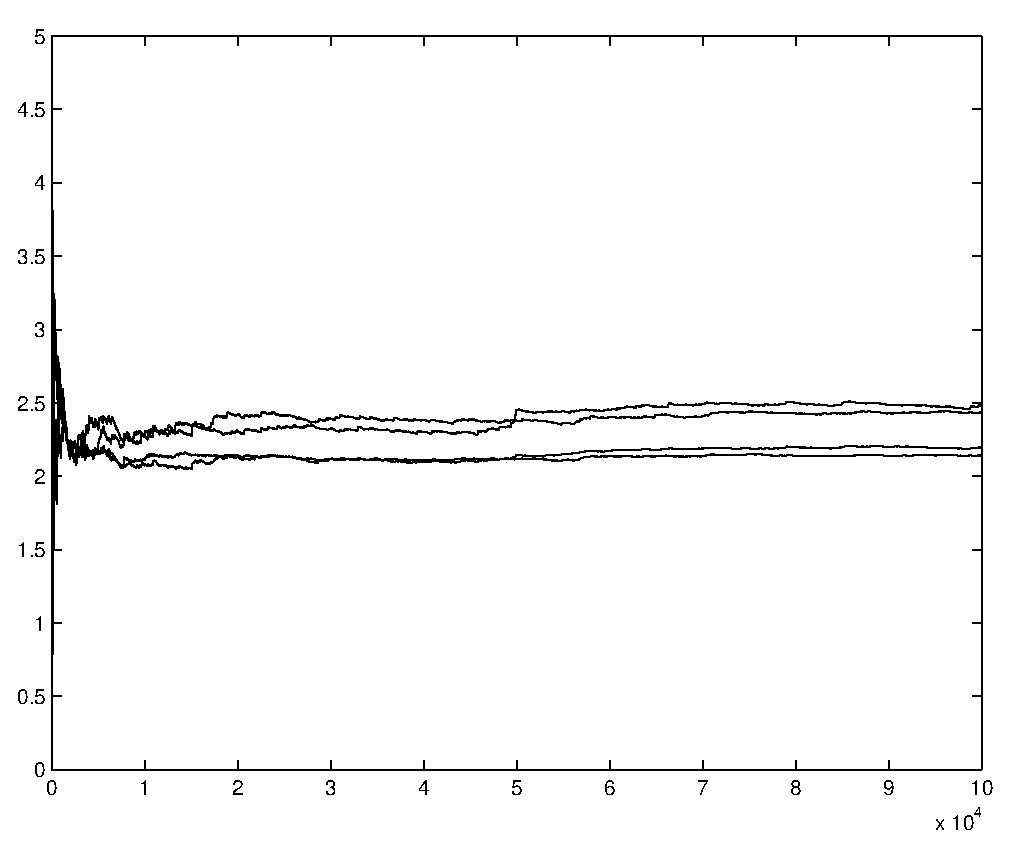
\includegraphics[height=6cm]{4bii.eps}
\caption{Figure of queue for question1}
\end{figure}
For the base case $\lambda_i=1.5$, $\mu=2$ as effectively all the
links are equal then for each link

$$
\rho=\frac{\lambda}{\mu}=\frac{1.5}{2}=0.75
$$

so
$$
\overline{Q}_Q=\frac{\rho^2}{1-\rho}=\frac{0.75^2}{1-0.75}=2.25
$$
\FloatBarrier

 What we actually get for each queue is

$ q_1=2.3838 $ \\ $ q_2=2.2715 $ \\ $ q_3=2.4447 $ \\ $ q_4=2.4761
$

Here the analytical calculations are quite close to the values
obtained in practice.
\subsection*{Question 3biii}
\begin{figure}[h]
\centering
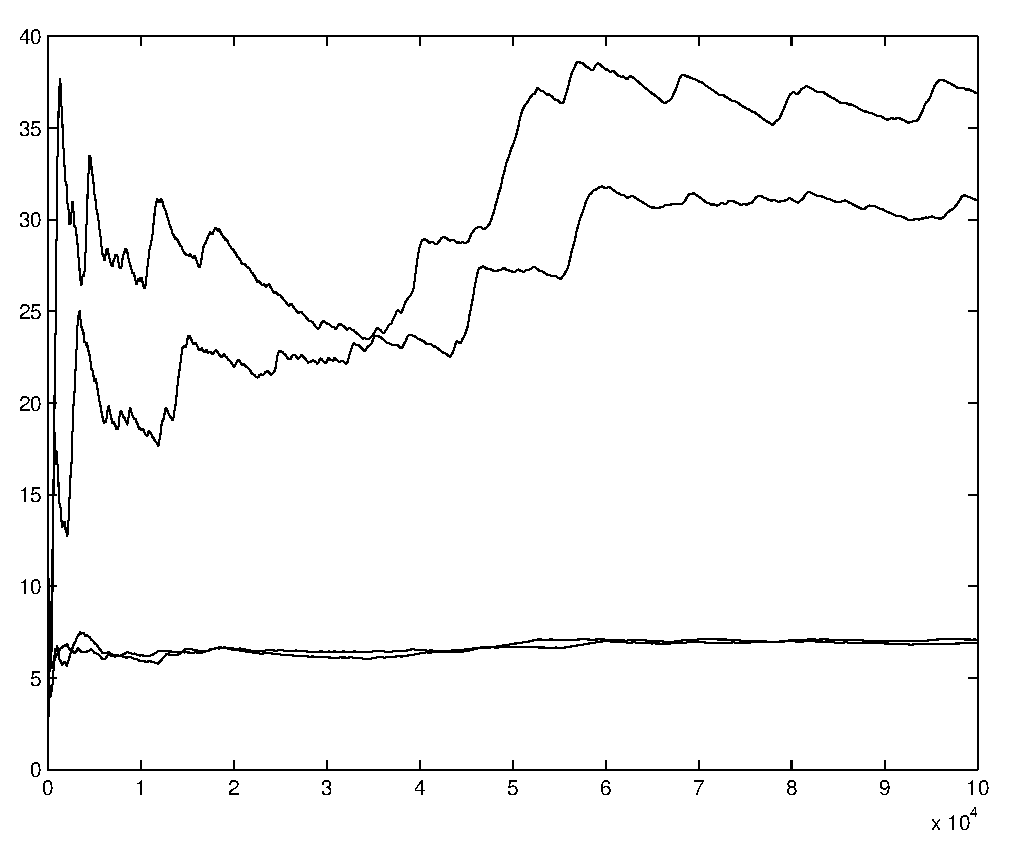
\includegraphics[height=6cm]{4biii.eps}
\caption{Figure of queue for question1}
\end{figure}
\FloatBarrier For the base case $\lambda_i=1.9$, $\mu=2$ as
effectively all the links are equal then for each link

$$
\rho=\frac{\lambda}{\mu}=\frac{1.9}{2}=0.95
$$

so
$$
\overline{Q}_Q=\frac{\rho^2}{1-\rho}=\frac{0.95^2}{1-0.95}=18.05
$$
What we actually get for each queue is

$ q_1=17.2824 $ \\ $ q_2=30.9351 $ \\ $ q_3=6.6866 $ \\ $
q_4=6.2884 $

First two quite good whereas the second to not so but we must take
into account Burkes theorem.
\subsection*{Question 3ci}
\begin{figure}[h]
\centering
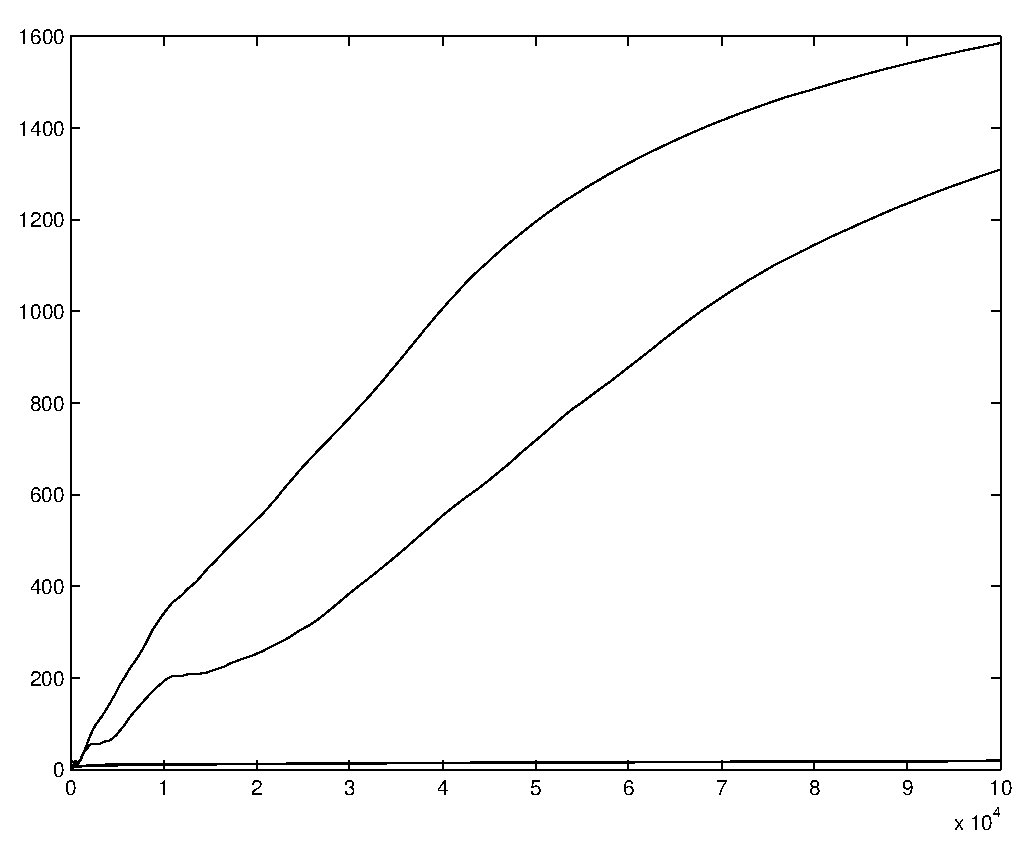
\includegraphics[height=6cm]{4ci.eps}
\caption{Figure of queue for question1}
\end{figure}
Consider that as the bandwidth has been halved then effectively
the value of mu has been halved as the death rate is effectively
halved. For the base case $\lambda_i=1$, $\mu=1$ as effectively
all the links are equal then for each link

$$
\rho=\frac{\lambda}{\mu}=\frac{1}{1}=1
$$

so
$$
\overline{Q}_Q=\frac{\rho^2}{1-\rho}=\frac{1^2}{1-1}=\infty
$$
\FloatBarrier Which means the queue gets effectively longer and
longer which from the intuition behind the values of lambda and mu
seems a sensible conclusion.
\subsection*{Question 3cii}
\begin{figure}[h]
\centering
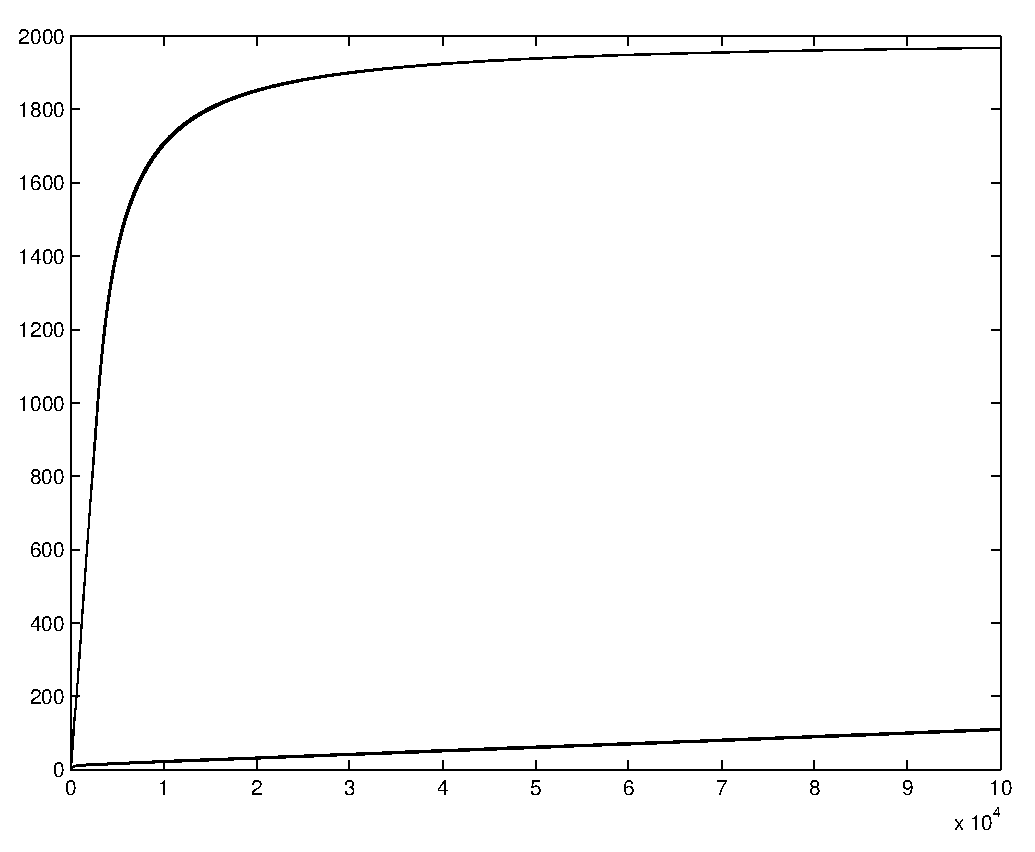
\includegraphics[height=6cm]{4cii.eps}
\caption{Figure of queue for question 4cii}
\end{figure}
Consider that as the bandwidth has been halved then effectively
the value of mu has been halved as the death rate is effectively
halved. For the base case $\lambda_i=1.5$, $\mu=1$ as effectively
all the links are equal then for each link

$$
\rho=\frac{\lambda}{\mu}=\frac{1.5}{1}=1.5
$$


so
$$
\overline{Q}_Q=\frac{\rho^2}{1-\rho}=\frac{1.5^2}{1-1.5}=-4.5
$$
\FloatBarrier Which means the queue gets effectively longer and
longer which from the intuition behind the values of lambda and mu
seems a sensible conclusion.
\subsection*{Question 3ciii}
\begin{figure}[h]
\centering
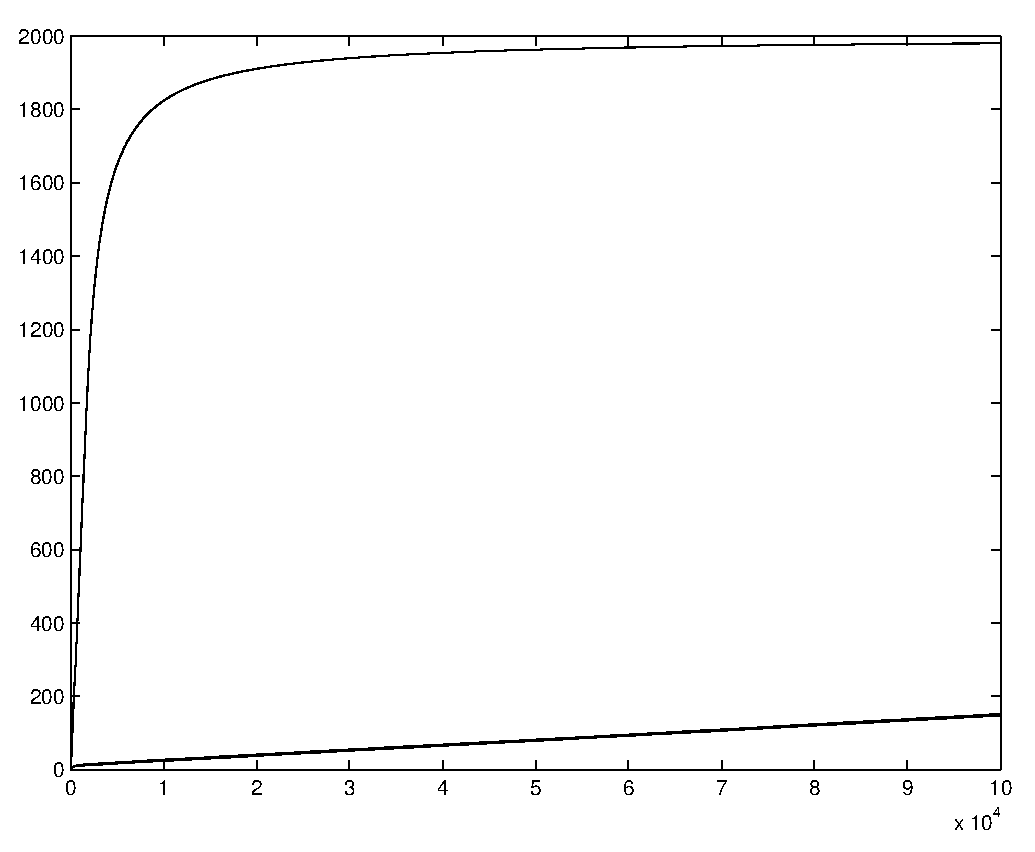
\includegraphics[height=6cm]{4ciii.eps}
\caption{Figure of queue for question3ciii}
\end{figure}
Consider that as the bandwidth has been halved then effectively
the value of mu has been halved as the death rate is effectively
halved. For the base case $\lambda_i=1.9$, $\mu=1$ as effectively
all the links are equal then for each link

$$
\rho=\frac{\lambda}{\mu}=\frac{1.9}{1}=1.9
$$


so
$$
\overline{Q}_Q=\frac{\rho^2}{1-\rho}=\frac{1.9^2}{1-1.9}=-4.01111
$$
Which means the queue gets effectively longer and longer which
from the intuition behind the values of lambda and mu seems a
sensible conclusion. So we can not model the queue accurately with
these equations.
\section*{Question 4}
These are advanced questions which were for the student to
discover in their own time if they were interested enough to do
so. As such they will not be covered here.
\end{document}
